%% This is an example first chapter.  It will help if you put the chapter/appendix that you
%% write into a separate file and add a line \include{yourfilename} to
%% main.tex, where `yourfilename.tex' is the name of the chapter/appendix file.
%% You can process specific files by typing their names in at the 
%% \files=
%% prompt when you run the file main.tex through LaTeX.

\chapter{Introduction}
Mercury (Hg) is a severe health hazard in the environment and for people, especially for fetuses and young children\cite{gibb_mercury_2014}. The release of mercury into the atmosphere results from human activities and natural processes. Upon release, mercury moves between the air, soils, and waters until, eventually, it is removed from the system through burial in coastal and deep ocean sediments, lake sediments, and subsurface soils \cite{esdaile_mercury_2018}. Moreover, mercury can travel great distances when released into the atmosphere, contaminating ecosystems, fish, birds, mammals, and human food chains \cite{esdaile_mercury_2018}. Recent estimates, as seen in Figure \ref{fig:gma2018_hg-emissions_by-industry},  indicate that about 37.7\% of global Hg emissions come from ASGM, making it the largest source of Hg pollution to the atmosphere and hydrosphere around the world\cite{united_nations_environment_programme_technical_2019}. However, the amount of Hg released by ASGM activities and the extent to which it is transported regionally and globally is highly uncertain. This thesis explores how top-down estimates of Hg emissions through atmospheric modeling would add value to the effectiveness evaluation of the MC on understanding ASGM Hg emission. 

\begin{figure}[H]
  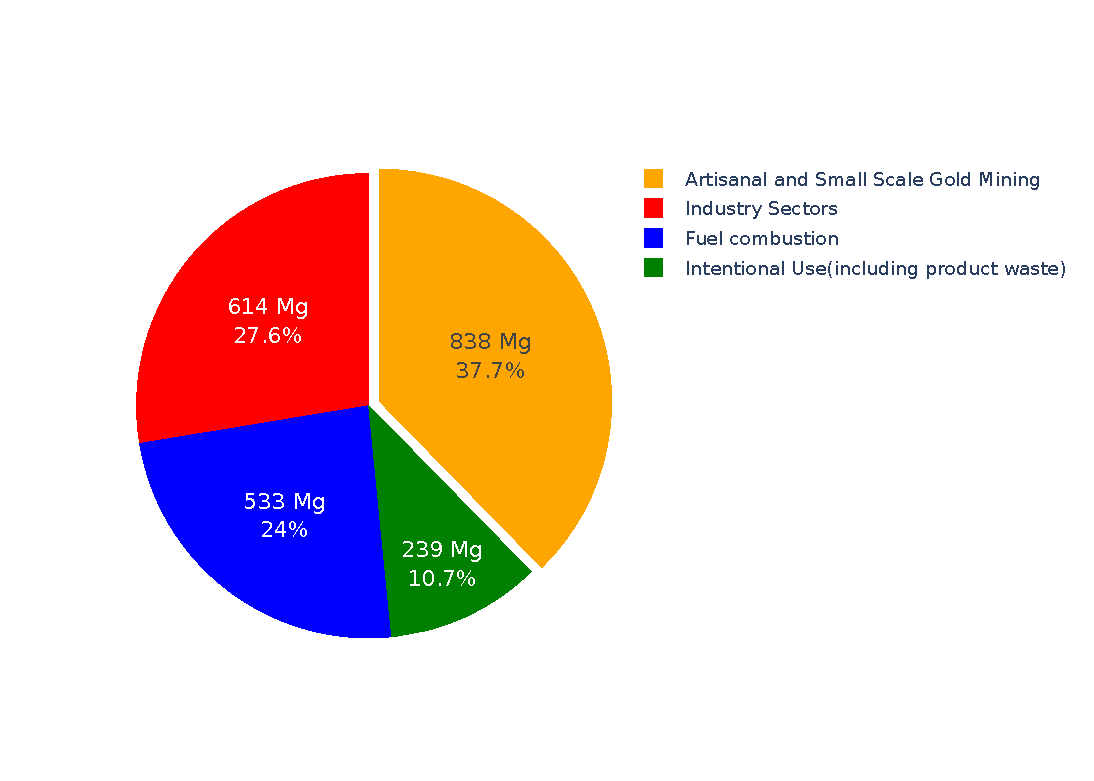
\includegraphics[width=0.8\textwidth]{templates/figures/07-24-22_gma2018_hg-emissions_by-industry.pdf}
  \centering
  \caption{Pie chart showing the 2018 global mercury assessment (GMA 2018) ASGM \hg emission estimates for different sectors. ASGM is the sector with the highest Hg emissions (shown in orange) at 838 Mg, followed by industry sectors (shown in red) at 614 Mg, then fuel combustion (shown in blue) at 533 Mg, and finally, intentional use sectors excluding ASGM (show in green) at 239 Mg \cite{united_nations_environment_programme_technical_2019}.}
  \label{fig:gma2018_hg-emissions_by-industry}
\end{figure}
\FloatBarrier

\section{Motivation}
\begin{flushleft}
While most of the Hg pollution from ASGM is local, its ability to travel across borders and contaminate distant ecosystems bolsters the case for concerted global efforts to eliminate Hg pollution in all forms, including ASGM Hg pollution. The Minamata Convention (MC) is a legally binding global treaty to protect human health and the environment from the adverse effects of mercury. Its text comprises articles that also target ASGM Hg emissions\cite{unep_minamata_2013}. Article 22 of the MC demonstrates the importance of consistent and scientifically rigorous reporting, including reporting from ASGM, about Hg releases and emissions, if sound policies and management actions are to be developed that promote sustainable change. 
\end{flushleft}
\begin{flushleft}
More than 100 million people depend on artisanal and small-scale gold mining (ASGM) for their livelihood globally, particularly in the over 81 countries, predominantly in the global south where ASGM exists\cite{planetgold_planetgold_2021}. Additionally, ASGM is an essential source of income and an opportunity for rural development in countries where options and alternatives to ASGM for generating income to buy necessities of daily life are in short supply or nonexistent \cite{planetgold_planetgold_2021}. It is estimated that around 10 to 20 million (ASGM) miners are employed in ASGM worldwide - about a third of them are women - and they provide 90\% of the global gold mining workforce and extract about 20\% of the world's gold annually \cite{planetgold_planetgold_2021}. For example, in Peru, ASGM sustains the livelihoods of an estimated 1 million people, and between 300,000 and 500,000 miners were involved in Peru's ASGM sector as of 2014. Despite being a vital source of livelihood for the communities that practice ASGM, its activities often lead to several environmental, human, and social harms. In addition to Hg releases to the environment, ASGM externalities include deforestation, tropical diseases such as malaria, dangerous and unsafe working conditions, crime and exploitation of indigenous communities, diesel and gasoline spills, and human trafficking \cite{usaid_usaid_2020}. 
\end{flushleft}

\section{Artisanal and Small-Scale Gold Mining}

\begin{flushleft} 
During ASGM, Hg is added to the gold ore to form a mercury-gold amalgam, a mixture of about equal amounts of Hg and gold\cite{united_nations_environment_programme_reducing_2012}. Heat is applied to the amalgam, which evaporates the Hg, leaving the gold behind. Gold extraction using this method is popular with the ASGM community since it is inexpensive, easy to use, and quick \cite{united_nations_environment_programme_reducing_2012}. Moreover, Hg is relatively effective at capturing gold when there are no alternatives but often captures less than 40\% \cite{united_nations_environment_programme_developing_2015}. There is usually a tremendous amount of Hg vapor in the air around amalgam burning sites, much higher than the World Health Organization(WHO) limit of 1.0 $\mu$g/m$^{3}$\cite{gibb_mercury_2014}. The Hg emissions in ASGM are harmful to miners and members of their communities.
Additionally, humans and ecosystems far away are also exposed to Hg risks because Hg travels globally through the atmosphere. As vaporized Hg settles in soil, rivers, bays, and oceans, anaerobic organisms transform it into methylmercury, and water bodies can become contaminated with methylmercury\cite{united_nations_environment_programme_technical_2019}. Methylmercury is absorbed and ingested by phytoplankton, zooplankton, and fish, and predator species such as sharks and swordfish that live a long time accumulate methylmercury and are usually the source of poisoning for people who eat fish\cite{gibb_mercury_2014}. Figure \ref{fig:world_hg_emisions} shows how the annual average of the total Hg emissions from  all global anthropogenic Hg emissions sources is distributed. 
\end{flushleft}

\begin{figure}[H]
  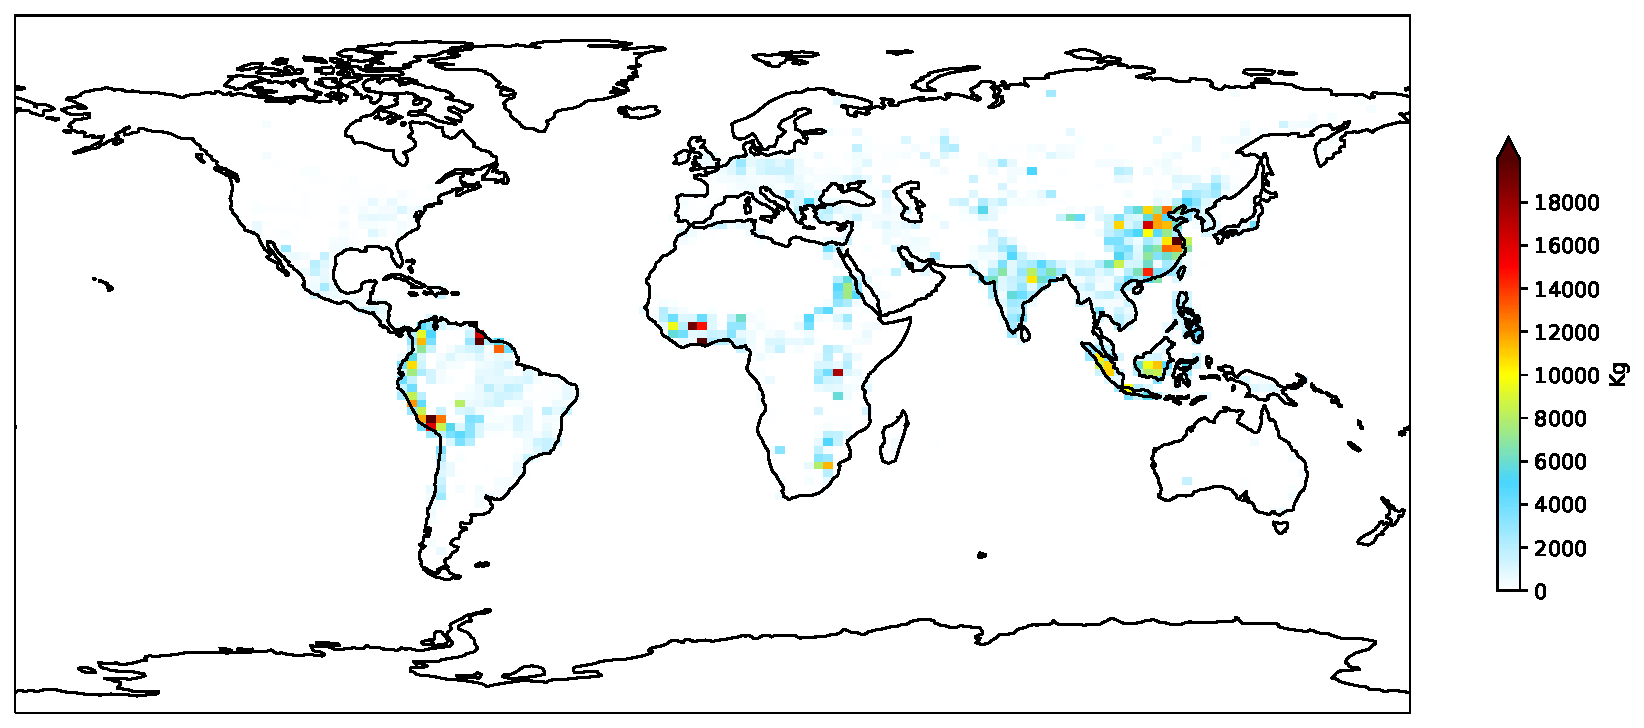
\includegraphics[width=0.8\textwidth]{templates/figures/06-12-22_total_Hg0-emissions-per-year_globally_001.pdf}
  \centering
  \caption{Spatial distribution of annual average Hg anthropogenic emissions for a year between July 2014 and July 2015 \cite{united_nations_environment_programme_technical_2019}}
  \label{fig:world_hg_emisions}
\end{figure}
\FloatBarrier

\section{ASGM Measures in the Minamata Convention}
\begin{flushleft}
    

The MC is a global treaty that was agreed upon at the fifth meeting of the Intergovernmental Negotiating Committee on Hg in Geneva, Switzerland, in January 2013 and formally adopted in October that year in Kumamoto, Japan. Moreover, the treaty entered into force on 16 August 2017, 90 days after the 50\textsuperscript{th} instrument of ratification was deposited, and currently has 137 parties to the convention\cite{unep_minamata_2013}. The MC's goal is to protect human health and the environment from the adverse effects of mercury, and it affirmed that global action is essential to address the Hg pollution problem. Article 7 and Annex C of the MC target ASGM. Article 7 requires countries where Hg is used in ASGM to develop a National Action Plan (NAP) that details ways to reduce and, where possible, eliminate the use of Hg and Hg compounds. Each country should include in its NAP actions to stop some of the worst practices of ASGM, which include, among other things, (i) whole ore amalgamation, (ii) open burning of amalgam, (iii) burning of amalgam in residential areas (iv), and cyanide leaching in sediment or tailings to which Hg has been added without first removing the Hg \cite{united_nations_environment_programme_technical_2019}.
Moreover, countries are required to include in their NAPs baseline estimates the quantities of Hg used in ASGM. The guidance document on developing a national action plan states that the goal should be to produce an estimate that has an accuracy of $\pm$ 30\% and, at worst, $\pm$ 50\%.  This is argued to be an obtainable level of confidence in the context of effort, time, and financial resources while being good enough to inform the NAP and allow for prioritization of actions \cite{unep_developing_2017}. A vital component of the MC is Article 22, which specifies a variety of information that must be included when conducting the effectiveness evaluation of the MC. The article states that "the Conference of the Parties shall, at its first meeting, initiate the establishment of arrangements for providing itself with comparable monitoring data on the presence and movement of Hg and Hg compounds in the environment as well as trends in levels of Hg and Hg compounds observed in biotic media and vulnerable populations." In addition, the MC secretariat recently published the monitoring guidance, which explains the role of monitoring in the effectiveness evaluation and sets realistic expectations about what can be learned over time, among other guidance goals \cite{unep_guidance_2021}. 
\end{flushleft}

\section{Case Study Region}
\begin{flushleft}
Latin America has the highest average ratio of mercury losses to gold production at 4.63, according to Yoshimura et al.'s (2021) estimate. Africa and Asia have the lowest at 1.96 and 1.23, respectively. Moreover, the GMA 2018 reported that ASGM Hg emissions in Latin America were the highest, and Figure \ref{fig:global_asgm_emissions_above_a_tone_barchart} shows that Peru is one of the top emitters of ASGM-related Hg and 60\% of the top 10 ASGM Hg emitting countries in the world are in Latin America  \cite{united_nations_environment_programme_technical_2019}. However, atmospheric Hg data from Latin America are rare; hence Hg dynamics in the region are not well understood. 
\end{flushleft}
\begin{figure}[H]
  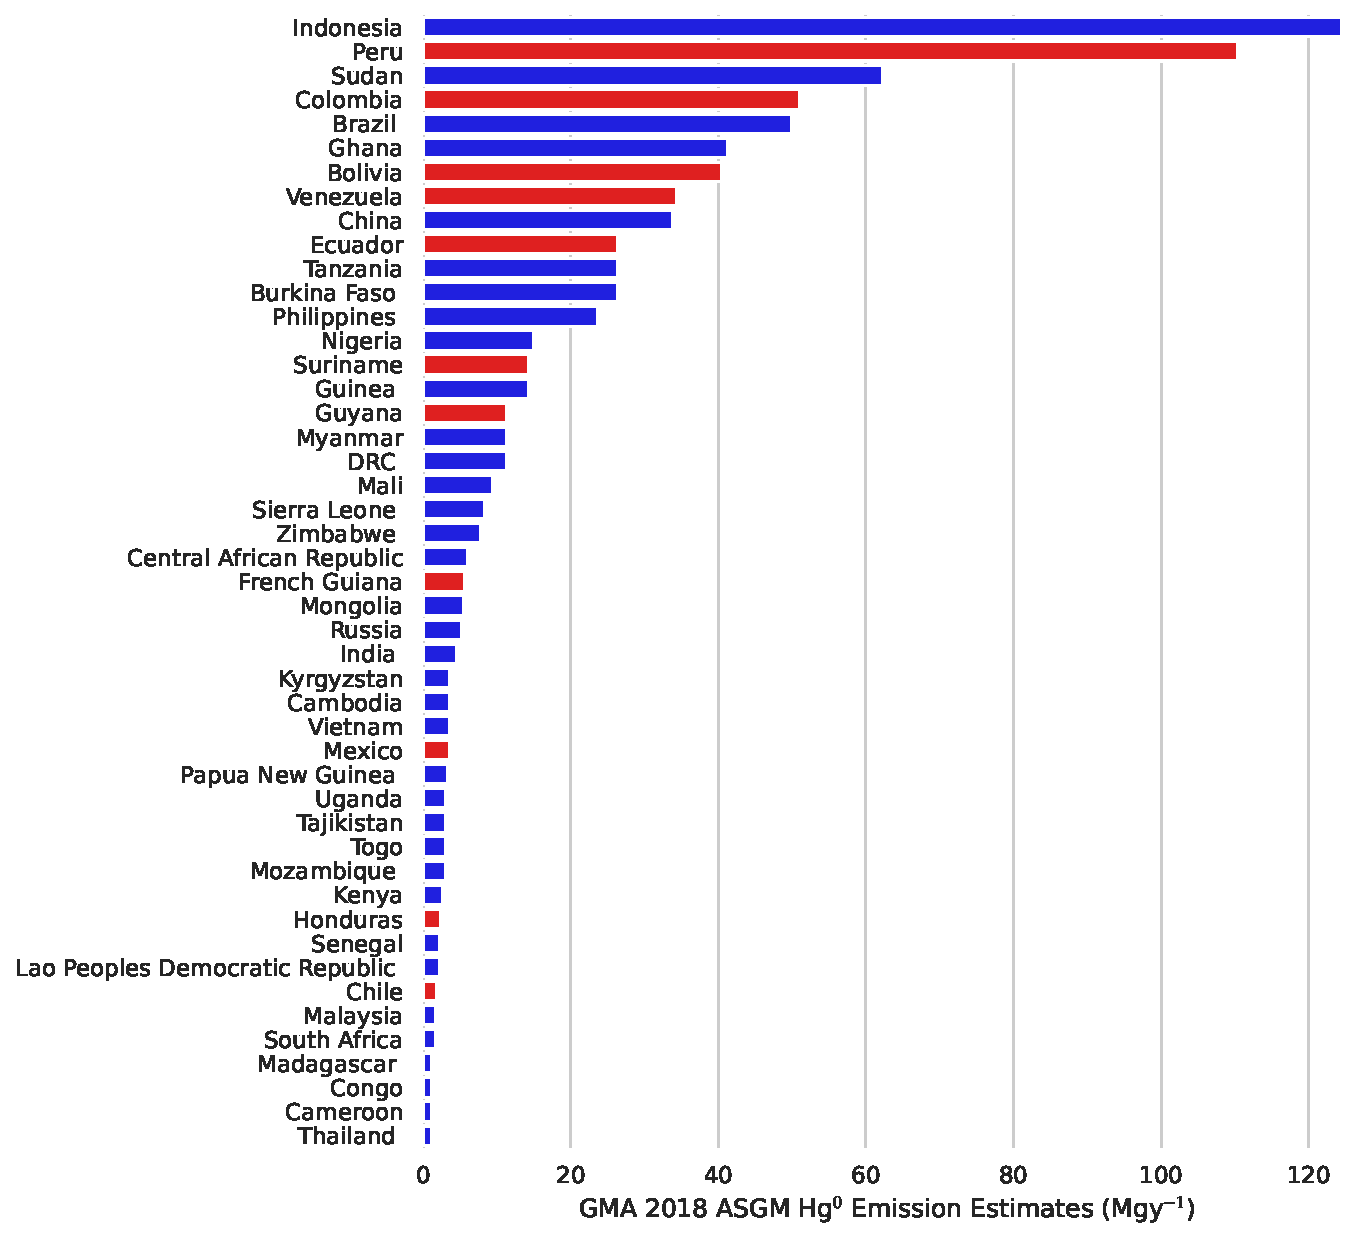
\includegraphics[width=\textwidth]{templates/figures/07-14-22_gma2018_top-asgm-emmiting-countries.pdf}
  \centering
  \caption{Bar chart showing the GMA 2018 ASGM \hg emission estimates for all countries worldwide that have estimated ASGM \hg emissions above 1 Mg. The red bars highlight countries in Latin America \cite{united_nations_environment_programme_technical_2019}}
  \label{fig:global_asgm_emissions_above_a_tone_barchart}
\end{figure}
\FloatBarrier
\begin{flushleft}
Additionally, Peru is the source of the largest ASGM emissions in Latin America, as seen in Figure \ref{fig:global_asgm_emissions_above_a_tone_barchart} and the Madre de Dios region in Peru was estimated to have released the largest quantities of Hg to the environment and the atmosphere\cite{agc_reporte_2017}. Madre de Dios, shown by the red outline in Figure \ref{fig:PeruCS}, is a rain-forest region between Bolivia and Brazil and covers roughly 85,000 square kilometers. The region's name is derived from the name of a major river that runs through it, and smaller streams and rivers cross through it to provide transportation and fishing for indigenous communities. Furthermore, these waterways are the main sites of ASGM and, subsequently, Hg contamination \cite{ashe_elevated_2012,agc_reporte_2017}. 
\begin{figure}[H]
  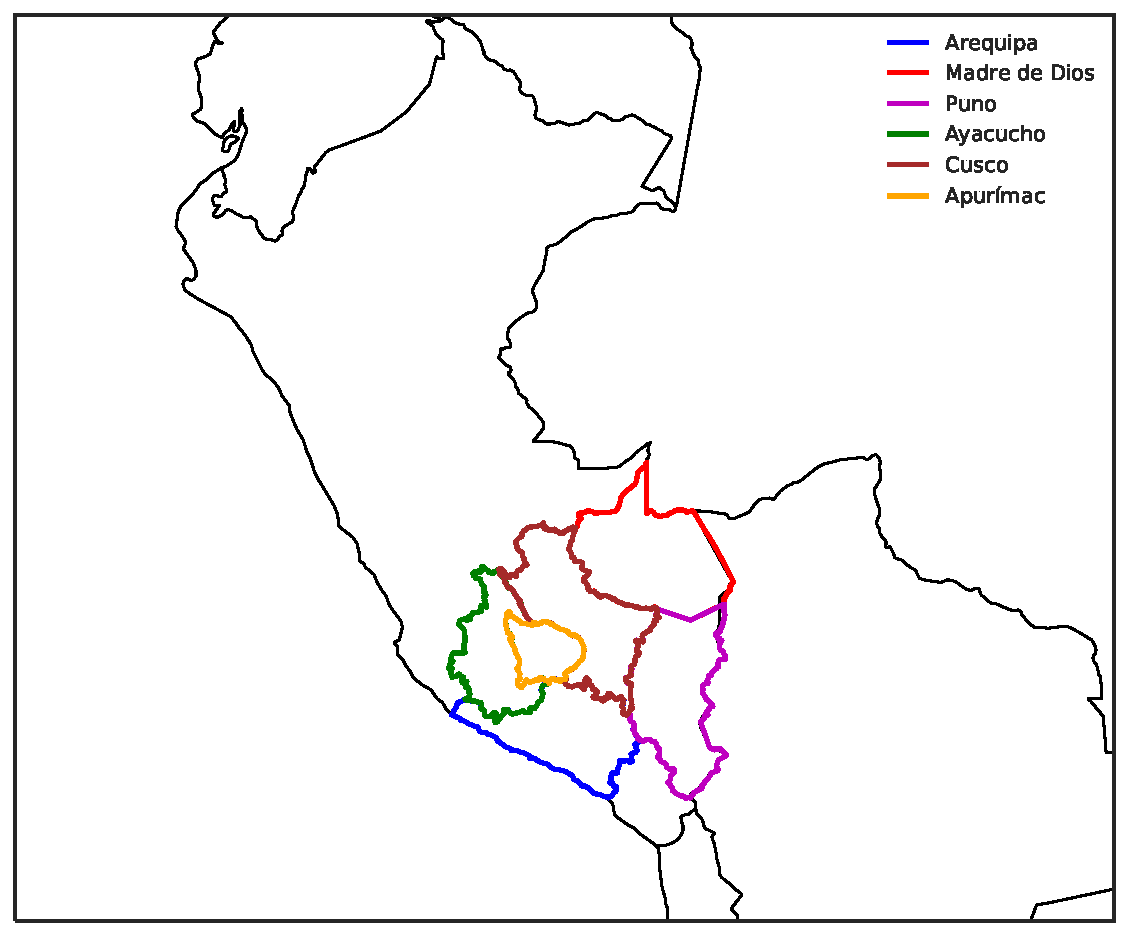
\includegraphics[width=0.6\textwidth]{templates/figures/Peru_Maps/CasestudyRegion.pdf}
  \centering
  \caption{Departments predicted to be the prominent sources of ASGM Hg releases according to the Artisanal Gold Council's  Inventory Report for the ASGM sector in Peru (2017) }
  \label{fig:PeruCS}
\end{figure}
\FloatBarrier

Hg has been extensively studied in Madre de Dios, in both people and the environment. This thesis project seeks to: 1) complement previous studies and distinguish itself  by investigating the extent to which the GEOS-Chem model can leverage existing measurements of Hg in the atmosphere, 2) determine bottom-up Hg emission estimates in published Hg global and national inventories to constrain the amount of ASGM Hg emissions from the case study region in Peru. 

\end{flushleft}
\begin{flushleft}


\section{Thesis Questions}
According to Evers et al.(2016), country-specific actions under Article 7 of the MC will differ from country to country, and this variability poses a challenge to assessing the MC's effectiveness. Additionally, they argue that changes in the overall use of Hg in the global ASGM sector can be informed by progress in individual countries. They suggest a compilation, visualization, and mapping of the respective data to track this progress across ASGM countries. Moreover, N.E Selin (2014) highlighted that the existing global-scale monitoring networks for background Hg levels could not indicate whether the MC would lead to changes in the global biogeochemical cycling of Hg. She further argued that monitoring policy effectiveness in reducing emissions and tracking potential changes requires better knowledge of and the ability to explain baseline levels in the global biogeochemical cycle without policy. The value added by baseline estimates of emissions to policy making is also recognized in the MC's paragraph 3 of Article 7, which stipulates that each party that notifies the secretariat that (ASGM) and processing in its territory is more than insignificant shall develop and implement a national action plan (NAP) per annex C to the MC. In addition, annex C (d) states that the NAP shall include baseline estimates of the quantities of Hg used and the practices employed in ASGM and processing. As of this writing, 18 countries have submitted their respective NAPs, and the estimates of how much Hg is used in their territories are shown in Figure\ref{fig:global-hg-emission-estimates_vs_nap_estimates}. 

\begin{figure}[H]
  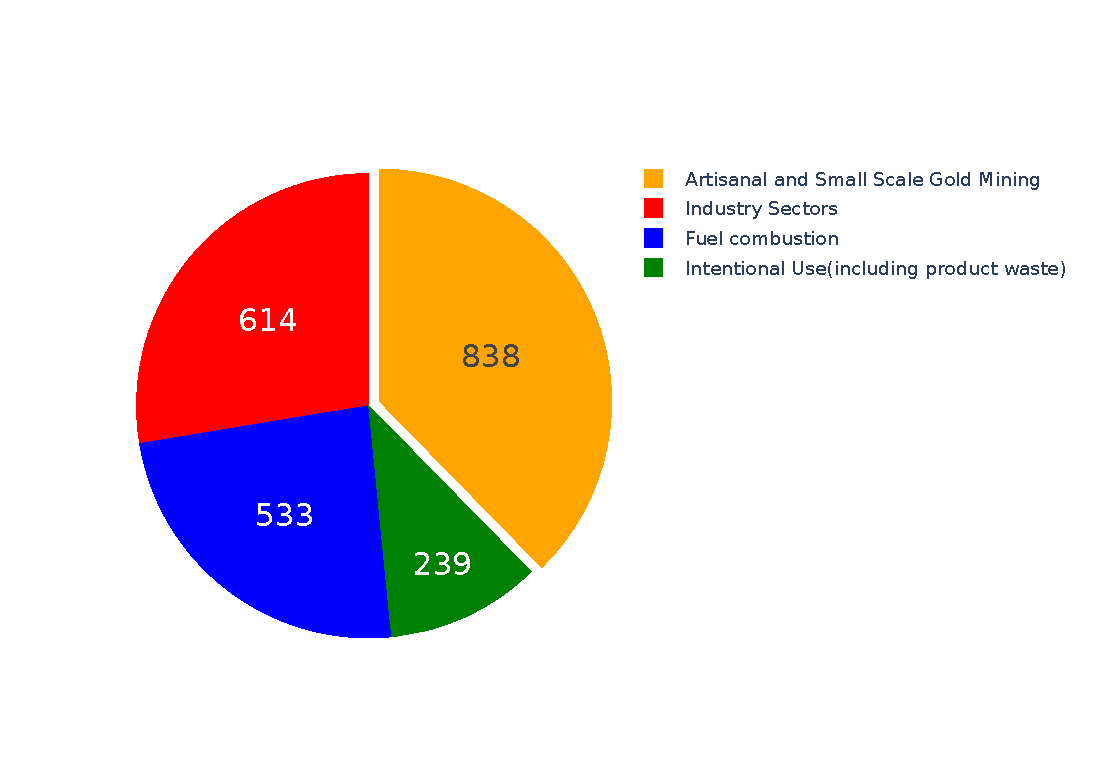
\includegraphics[width=\textwidth]{templates/figures/07-24-22_global-hg-emission-estimates_vs_nap_estimates.pdf}
  \centering
  \caption{Bar chart comparing the estimates of annual average Hg emissions predicted in the GMA 2018 inventory in light blue vs. annual average Hg emissions baseline estimates (shown in dark blue) that were reported by the respective countries in their NAPs \cite{united_nations_environment_programme_technical_2019} }
  \label{fig:global-hg-emission-estimates_vs_nap_estimates}
\end{figure}
\FloatBarrier


 It is evident, in Figure \ref{fig:global-hg-emission-estimates_vs_nap_estimates}, that the difference between the global estimates and the NAP estimates is vast for some countries. While the baseline estimates of Hg use in ASGM as reported in the NAPs and global inventories are critical, data from monitoring networks combined with atmospheric models provide additional tools to evaluate the changes in Hg in the atmosphere. Several studies have identified atmospheric mercury monitoring as a primary and appropriate method to assess the effectiveness of the MC\cite{sprovieri_atmospheric_2016,evers_evaluating_2016,gustin_measuring_2015,united_nations_environment_programme_technical_2019}. Likewise, the monitoring guidance,\cite{unep_guidance_2021} echoes this by emphasizing the provision of data for the development and improvement of transport and chemistry models as one of the primary objectives of monitoring Hg in the atmosphere. Nevertheless, few studies have demonstrated how models can inform policy on ASGM Hg emissions using monitoring data. Consequently, I aim to answer the following questions based on the assumption that using chemical transport models (CTMs) such as GEOS-Chem can provide a means to synthesize data from national and global Hg inventories and atmospheric monitoring networks to track progress and measure MC's effectiveness:
\begin{enumerate}
  \item To what extent can regional atmospheric modeling and monitoring help reconcile the differences in the current global estimates of emissions and national emissions?
  \item What regional monitoring networks are essential to improve the utility of models in evaluating the MC's effectiveness?
  \item Which policies are essential to catalyzing action towards the expansion of regional monitoring, particularly in the regions where ASGM emissions are the dominant source?
\end{enumerate}
\end{flushleft}




 
\section{Organization}
 
\begin{flushleft}
  This introductory chapter has provided a general background on ASGM concerning Hg emissions and the extent of global efforts to protect people and the environment from the adverse effects of Hg pollution. Chapter 2 addresses the first thesis question by evaluating GEOS-Chem modeled atmospheric Hg concentrations across Latin America with observed Hg concentrations at various regional sites. The strengths and limitations of the GEOS-Chem model are highlighted, and strategies to improve the model's usefulness are discussed. Chapter 3 addresses the second question by presenting a method to produce top-down estimates of ASGM Hg emissions and discussing possible network configurations to monitor ASGM Hg emissions. Finally, chapter 4 presents policy recommendations and conclusions to address the third research question.  
\end{flushleft}



%\section{Organization}